% answers.tex —— 2021 年·全国甲卷·理科 · 参考答案与详细解析片段
% 由 tools/generate_projects.py 依来源总账自 2021/2021_数学真题_全国甲理_试题.md + 2021/2021_数学真题_全国甲理_解析正文.md + 2021/2021_数学真题_全国甲理_答案要点.md 生成，勿手改（改源 MD 后重跑）


\begin{gknotice}
\textbf{解析归属}：以下推导根据固定上游题面独立重建，不是官方答案、官方解析或评分细则。
\end{gknotice}

\gkpart{一、选择题}

\begin{answer}
\gksolhead{1}{}

\textbf{题目}：

设集合 $M=\{x\mid 0<x<4\}$，$N=\left\{x\mid \dfrac13\leqslant x\leqslant5\right\}$，则 $M\cap N=$\mbox{（　　）}

\begin{gkopts}(2)
\task A．$\left\{x\mid 0<x\leqslant\dfrac13\right\}$
\task B．$\left\{x\mid\dfrac13\leqslant x<4\right\}$
\task C．$\{x\mid4\leqslant x<5\}$
\task D．$\{x\mid0<x\leqslant5\}$
\end{gkopts}

\Needspace{4\baselineskip}
\textbf{解析}

$M$ 的范围是 $0<x<4$，$N$ 的范围是 $\dfrac13\leqslant x\leqslant5$。取交集得 $\dfrac13\leqslant x<4$，对应 B。

\gkanswer{答案：B}

\end{answer}
\begin{answer}
\gksolhead{2}{}

\textbf{题目}：

为了解某地农村经济情况，对该地农户家庭年收入进行抽样调查，将农户家庭年收入的调查数据整理得到如下频率分布直方图：
\nopagebreak[4]
\begin{center}% 2021 全国甲卷理科 2：农村家庭年收入频率分布直方图
% 根据固定上游 PDF 第 1 页：组距均为 1，组界 2.5 至 14.5。
% 各柱高依次为 0.02, 0.04, 0.10, 0.14, 0.20, 0.20, 0.10, 0.10, 0.04, 0.02, 0.02, 0.02。
\begin{tikzpicture}[font=\small]
  \def\xs{0.48}\def\ys{15.0}\def\xz{0.52}
  % 横轴断轴与纵轴
  \draw (0,0) -- (0.10,0);
  \draw (0.10,0) -- (0.16,0.09) -- (0.25,-0.09) -- (0.31,0);
  \draw[->] (0.31,0) -- ({\xz+12*\xs+0.55},0);
  \draw[->] (0,0) -- (0,{0.20*\ys+0.45});
  \node[anchor=north] at (0,-0.04) {$0$};
  \node[anchor=south east,align=center] at (-0.04,{0.20*\ys+0.1}) {频率/组距};
  \node[anchor=west] at ({\xz+12*\xs+0.2},0.15) {收入/万元};
  % 刻度参考线及标注
  \foreach \v in {0.02,0.04,0.10,0.14,0.20} {
    \draw[densely dotted,gray!70] (0,{\v*\ys}) -- ({\xz+12*\xs},{\v*\ys});
    \node[anchor=east,inner sep=2pt,font=\scriptsize] at (-0.04,{\v*\ys}) {$\v$};
  }
  % 十二组柱形
  \foreach \i/\h in {0/0.02,1/0.04,2/0.10,3/0.14,4/0.20,5/0.20,
                       6/0.10,7/0.10,8/0.04,9/0.02,10/0.02,11/0.02} {
    \draw ({\xz+\i*\xs},0) rectangle ({\xz+(\i+1)*\xs},{\h*\ys});
  }
  \foreach \i/\xlab in {0/2.5,1/3.5,2/4.5,3/5.5,4/6.5,5/7.5,6/8.5,
                         7/9.5,8/10.5,9/11.5,10/12.5,11/13.5,12/14.5} {
    \node[anchor=north,inner sep=1pt,font=\tiny] at ({\xz+\i*\xs},-0.04) {$\xlab$};
  }
\end{tikzpicture}
\end{center}
\nopagebreak[4]
根据此频率分布直方图，下面结论中不正确的是\mbox{（　　）}

\begin{gkopts}(1)
\task A．该地农户家庭年收入低于 $4.5$ 万元的农户比率估计为 $6\%$
\task B．该地农户家庭年收入不低于 $10.5$ 万元的农户比率估计为 $10\%$
\task C．估计该地农户家庭年收入的平均值不超过 $6.5$ 万元
\task D．估计该地有一半以上的农户，其家庭年收入介于 $4.5$ 万元至 $8.5$ 万元之间
\end{gkopts}

\Needspace{4\baselineskip}
\textbf{解析}

\Needspace{5\baselineskip}
从 $2.5$ 到 $14.5$ 的 12 个组距均为 $1$，各组高度依次为
\nopagebreak[4]
\[
\begin{aligned}
&0.02,0.04,0.10,0.14,0.20,0.20,\\
&0.10,0.10,0.04,0.02,0.02,0.02.
\end{aligned}
\]
总频率为 $1$。

低于 $4.5$ 万元的频率为 $0.02+0.04=0.06$；不低于 $10.5$ 万元的频率为 $0.04+0.02+0.02+0.02=0.10$；$4.5$ 至 $8.5$ 万元的频率为 $0.10+0.14+0.20+0.20=0.64$。

\Needspace{5\baselineskip}
用各组中值加权，均值估计为
\nopagebreak[4]
\[
\begin{aligned}
3(0.02)+4(0.04)+5(0.10)+6(0.14)+7(0.20)+8(0.20)\\
+9(0.10)+10(0.10)+11(0.04)+12(0.02)+13(0.02)+14(0.02)=7.68.
\end{aligned}
\]
所以 C 所述“不超过 $6.5$ 万元”不正确。

\gkanswer{答案：C}

\end{answer}
\begin{answer}
\gksolhead{3}{}

\textbf{题目}：

已知 $(1-\mathrm i)^2z=3+2\mathrm i$，则 $z=$\mbox{（　　）}

\begin{gkopts}(2)
\task A．$-1-\dfrac32\mathrm i$
\task B．$-1+\dfrac32\mathrm i$
\task C．$-\dfrac32+\mathrm i$
\task D．$-\dfrac32-\mathrm i$
\end{gkopts}

\Needspace{4\baselineskip}
\textbf{解析}

\Needspace{5\baselineskip}
$(1-\mathrm i)^2=-2\mathrm i$，从而
\nopagebreak[4]
\[
z=\frac{3+2\mathrm i}{-2\mathrm i}
=\frac{(3+2\mathrm i)\mathrm i}{2}
=-1+\frac32\mathrm i.
\]
对应 B。

\gkanswer{答案：B}

\end{answer}
\begin{answer}
\gksolhead{4}{}

\textbf{题目}：

青少年视力是社会普遍关注的问题，视力情况可借助视力表测量。通常用五分记录法和小数记录法记录视力数据，五分记录法的数据 $L$ 和小数记录法的数据 $V$ 满足 $L=5+\lg V$。已知某同学视力的五分记录分的数据为 $4.9$，则其视力的小数记录法的数据约为（$\sqrt[10]{10}\approx1.259$）\mbox{（　　）}

\begin{gkopts}(4)
\task A．$1.5$
\task B．$1.2$
\task C．$0.8$
\task D．$0.6$
\end{gkopts}

\Needspace{4\baselineskip}
\textbf{解析}

\Needspace{5\baselineskip}
由 $4.9=5+\lg V$ 得 $\lg V=-0.1$，所以
\nopagebreak[4]
\[
V=10^{-0.1}=\frac1{\sqrt[10]{10}}\approx\frac1{1.259}\approx0.794.
\]
最接近的选项为 $0.8$，即 C。

\gkanswer{答案：C}

\end{answer}
\begin{answer}
\gksolhead{5}{}

\textbf{题目}：

已知 $F_1$，$F_2$ 是双曲线 $C$ 的两个焦点，$P$ 为 $C$ 上一点，且 $\angle F_1PF_2=60^\circ$，$|PF_1|=3|PF_2|$，则 $C$ 的离心率为\mbox{（　　）}

\begin{gkopts}(2)
\task A．$\dfrac{\sqrt7}{2}$
\task B．$\dfrac{\sqrt{13}}2$
\task C．$\sqrt7$
\task D．$\sqrt{13}$
\end{gkopts}

\Needspace{4\baselineskip}
\textbf{解析}

\Needspace{5\baselineskip}
令 $|PF_2|=r$，则 $|PF_1|=3r$。焦点间距离为 $2c$。在 $\triangle F_1PF_2$ 中用余弦定理：
\nopagebreak[4]
\[
(2c)^2=(3r)^2+r^2-2(3r)(r)\cos60^\circ=7r^2.
\]
双曲线焦点差为 $|PF_1|-|PF_2|=2a$，故 $2a=2r$，即 $a=r$。因此 $e=c/a=\sqrt7/2$，选 A。

\gkanswer{答案：A}

\end{answer}
\begin{answer}
\gksolhead{6}{}

\textbf{题目}：

在一个正方体中，过顶点 $A$ 的三条棱的中点分别为 $E$，$F$，$G$。该正方体截去三棱锥 $A\text{-}EFG$ 后，所得多面体的三视图中，正视图如图所示，则相应的侧视图是\mbox{（　　）}
\nopagebreak[4]
\begin{center}% 2021 全国甲卷理科 6：正视图与四个备选侧视图
% 依据固定上游 PDF 第 1 页。切口投影均落在方形边的中点；虚线/实线按遮挡关系区分。
\begin{tikzpicture}[font=\small,line width=0.4pt]
  \def\s{1.38}
  \newcommand{\cutleft}[1][]{\draw[#1] (0,{0.5*\s}) -- ({0.5*\s},0);}
  \newcommand{\cutright}[1][]{\draw[#1] ({0.5*\s},0) -- (\s,{0.5*\s});}
  % 正视图
  \begin{scope}[shift={({2.15*\s},{1.18*\s})}]
    \draw (0,0) rectangle (\s,\s);
    \cutleft[dashed]
    \node[anchor=south] at ({0.5*\s},\s+0.04) {正视图};
  \end{scope}
  % A：右下角、实线
  \begin{scope}[shift={(0,0)}]
    \draw (0,0) rectangle (\s,\s); \cutright
    \node[anchor=east] at (-0.05,{0.06*\s}) {A};
  \end{scope}
  % B：左下角、虚线
  \begin{scope}[shift={({1.55*\s},0)}]
    \draw (0,0) rectangle (\s,\s); \cutleft[dashed]
    \node[anchor=east] at (-0.05,{0.06*\s}) {B};
  \end{scope}
  % C：右下角、虚线
  \begin{scope}[shift={({3.10*\s},0)}]
    \draw (0,0) rectangle (\s,\s); \cutright[dashed]
    \node[anchor=east] at (-0.05,{0.06*\s}) {C};
  \end{scope}
  % D：左下角、实线
  \begin{scope}[shift={({4.65*\s},0)}]
    \draw (0,0) rectangle (\s,\s); \cutleft
    \node[anchor=east] at (-0.05,{0.06*\s}) {D};
  \end{scope}
\end{tikzpicture}
\end{center}
\nopagebreak[4]
\Needspace{4\baselineskip}
\textbf{解析}

截去顶点 $A$ 处的三棱锥后，截面与三条棱的交点均为中点。正视图中截面投影切去左下角，且该截边被遮挡，应画虚线。按通常三视图的左视图方向观察，该截角位于可见侧面，截边可见，应画实线，故选 D；若从右侧观察则截边为虚线，对应 C，不是这里的标准左视图。

\gkanswer{答案：D}

\end{answer}
\begin{answer}
\gksolhead{7}{}

\textbf{题目}：

等比数列 $\{a_n\}$ 的公比为 $q$，前 $n$ 项和为 $S_n$。设甲：$q>0$，乙：$\{S_n\}$ 是递增数列，则\mbox{（　　）}

\begin{gkopts}(2)
\task A．甲是乙的充分条件但不是必要条件
\task B．甲是乙的必要条件但不是充分条件
\task C．甲是乙的充要条件
\task D．甲既不是乙的充分条件也不是乙的必要条件
\end{gkopts}

\Needspace{4\baselineskip}
\textbf{解析}

\Needspace{5\baselineskip}
若 $\{S_n\}$ 递增，则对每个 $n$ 都有
\nopagebreak[4]
\[
a_{n+1}=S_{n+1}-S_n>0,
\]
于是 $q=a_{n+2}/a_{n+1}>0$，所以甲是乙的必要条件。

$q>0$ 并不足够：例如令 $a_1<0$ 且 $q>0$，则所有 $a_n<0$，$S_n$ 递减。故甲不是乙的充分条件，选 B。

\gkanswer{答案：B}

\end{answer}
\begin{answer}
\gksolhead{8}{}

\textbf{题目}：

2020 年 12 月 8 日，中国和尼泊尔联合公布珠穆朗玛峰最新高程为 $8848.86$（单位：m）。三角高程测量法是珠峰高程测量方法之一。如图是三角高程测量法的一个示意图，现有 $A$，$B$，$C$ 三点，且 $A$，$B$，$C$ 在同一水平面上的投影 $A'$，$B'$，$C'$ 满足 $\angle A'C'B'=45^\circ$，$\angle A'B'C'=60^\circ$。由 $C$ 点测得 $B$ 点的仰角为 $15^\circ$，$BB'$ 与 $CC'$ 的差为 $100$；由 $B$ 点测得 $A$ 点的仰角为 $45^\circ$，则 $A$，$C$ 两点到水平面 $A'B'C'$ 的高度差 $AA'-CC'$ 约为（$\sqrt3\approx1.732$）\mbox{（　　）}
\nopagebreak[4]
\begin{center}% 2021 全国甲卷理科 8：珠峰三角高程测量示意图
% 依据固定上游 PDF 第 1 页；地面投影、竖直高度及仰视线均按原图关系示意。
\begin{tikzpicture}[font=\small,line width=0.45pt,
  x={(0.78cm,0cm)},y={(0cm,0.72cm)},z={(0.32cm,0.20cm)}]
  % 地面投影构成角 A'C'B'=45°, A'B'C'=60° 的三角形（非等比例排版）
  \coordinate (Ap) at (0,0,0);
  \coordinate (Bp) at (4,0,0);
  \coordinate (Cp) at (1.268,0,4.732);
  % 三点位于投影上方；高度仅用于示意
  \coordinate (A) at (0,6.2,0);
  \coordinate (B) at (4,2.464,0);
  \coordinate (C) at (1.268,1,4.732);
  % 地面投影及高度垂线
  \draw (Ap)--(Bp)--(Cp)--cycle;
  \draw[dashed] (Ap)--(A) (Bp)--(B) (Cp)--(C);
  % 测量视线
  \draw (B)--(A);
  \draw (C)--(B);
  % 仰角/地面角文字标注
  \node at (2.0,4.3,0) {$45^\circ$};
  \node at (3.65,2.9,0) {$15^\circ$};
  \node at (2.4,0.8,0) {$45^\circ$};
  \node at (3.6,0.5,0) {$60^\circ$};
  % 高度差标注
  \node[anchor=west] at (5.1,3.2,0) {$BB'-CC'=100$};
  \node[anchor=east] at (-0.1,3.0,0) {$AA'-CC'$};
  % 点名
  \node[anchor=south] at (A) {$A$};
  \node[anchor=west] at (B) {$B$};
  \node[anchor=west] at (C) {$C$};
  \node[anchor=north east] at (Ap) {$A'$};
  \node[anchor=north west] at (Bp) {$B'$};
  \node[anchor=south east] at (Cp) {$C'$};
\end{tikzpicture}
\end{center}
\nopagebreak[4]
\begin{gkopts}(4)
\task A．$346$
\task B．$373$
\task C．$446$
\task D．$473$
\end{gkopts}

\Needspace{4\baselineskip}
\textbf{解析}

\Needspace{5\baselineskip}
设 $d=C'B'$。由 $C$ 到 $B$ 的仰角及高度差，
\nopagebreak[4]
\[
\tan15^\circ=\frac{100}{d},\qquad d=100\cot15^\circ=100(2+\sqrt3).
\]
\Needspace{5\baselineskip}
在水平投影三角形中，第三角为 $75^\circ$。正弦定理给出
\nopagebreak[4]
\[
A'B'=d\frac{\sin45^\circ}{\sin75^\circ}
=100(2+\sqrt3)(\sqrt3-1)=100(1+\sqrt3).
\]
\Needspace{5\baselineskip}
由 $B$ 看向 $A$ 的仰角为 $45^\circ$，所以 $AA'-BB'=A'B'$。再加上 $BB'-CC'=100$：
\nopagebreak[4]
\[
AA'-CC'=A'B'+100=100(2+\sqrt3)\approx373.2\text{ m}.
\]
按题目选项取 B。

\gkanswer{答案：B}

\end{answer}
\begin{answer}
\gksolhead{9}{}

\textbf{题目}：

若 $\alpha\in\left(0,\dfrac\pi2\right)$，$\tan2\alpha=\dfrac{\cos\alpha}{2-\sin\alpha}$，则 $\tan\alpha=$\mbox{（　　）}

\begin{gkopts}(2)
\task A．$\dfrac{\sqrt{15}}{15}$
\task B．$\dfrac{\sqrt5}{5}$
\task C．$\dfrac{\sqrt5}{3}$
\task D．$\dfrac{\sqrt{15}}5$
\end{gkopts}

\Needspace{4\baselineskip}
\textbf{解析}

\Needspace{5\baselineskip}
令 $s=\sin\alpha$。因 $0<\alpha<\pi/2$，$\cos\alpha>0$。将
\nopagebreak[4]
\[
\frac{2\sin\alpha\cos\alpha}{1-2\sin^2\alpha}
=\frac{\cos\alpha}{2-\sin\alpha}
\]
\Needspace{5\baselineskip}
约去 $\cos\alpha$ 并交叉相乘，得 $2s(2-s)=1-2s^2$，即 $s=1/4$。故
\nopagebreak[4]
\[
\tan\alpha=\frac{1/4}{\sqrt{15}/4}=\frac{\sqrt{15}}{15},
\]
选 A。

\gkanswer{答案：A}

\end{answer}
\begin{answer}
\gksolhead{10}{}

\textbf{题目}：

将 $4$ 个 $1$ 和 $2$ 个 $0$ 随机排成一行，则 $2$ 个 $0$ 不相邻的概率为\mbox{（　　）}

\begin{gkopts}(4)
\task A．$\dfrac13$
\task B．$\dfrac25$
\task C．$\dfrac23$
\task D．$\dfrac45$
\end{gkopts}

\Needspace{4\baselineskip}
\textbf{解析}

两个零在 6 个位置中任选 2 个，共 $\binom62=15$ 种等可能排法。相邻位置对有 5 种，故不相邻的排法有 $15-5=10$ 种，概率为 $10/15=2/3$，选 C。

\gkanswer{答案：C}

\end{answer}
\begin{answer}
\gksolhead{11}{}

\textbf{题目}：

已知 $A$，$B$，$C$ 是半径为 $1$ 的球 $O$ 的球面上的三个点，且 $AC\perp BC$，$AC=BC=1$，则三棱锥 $O\text{-}ABC$ 的体积为\mbox{（　　）}

\begin{gkopts}(2)
\task A．$\dfrac{\sqrt2}{12}$
\task B．$\dfrac{\sqrt3}{12}$
\task C．$\dfrac{\sqrt2}{4}$
\task D．$\dfrac{\sqrt3}{12}$
\end{gkopts}

\Needspace{4\baselineskip}
\textbf{解析}

\Needspace{5\baselineskip}
$AC\perp BC$ 且 $AC=BC=1$，所以 $\triangle ABC$ 面积为 $1/2$，斜边 $AB=\sqrt2$，其外接圆半径为 $\sqrt2/2$。平面 $ABC$ 截单位球所得圆的圆心是球心 $O$ 在该平面上的投影，因此球心到平面的距离为
\nopagebreak[4]
\[
h=\sqrt{1-\left(\frac{\sqrt2}{2}\right)^2}=\frac1{\sqrt2}.
\]
\Needspace{5\baselineskip}
四面体体积为
\nopagebreak[4]
\[
V=\frac13\cdot\frac12\cdot\frac1{\sqrt2}=\frac{\sqrt2}{12},
\]
选 A。原题 B、D 两个选项按题面图像均印作 $\sqrt3/12$，此处照录。

\gkanswer{答案：A}

\end{answer}
\begin{answer}
\gksolhead{12}{}

\textbf{题目}：

设函数 $f(x)$ 的定义域为 $\mathbf R$，$f(x+1)$ 为奇函数，$f(x+2)$ 为偶函数。当 $x\in[1,2]$ 时，$f(x)=ax^2+b$。若 $f(0)+f(3)=6$，则 $f\left(\dfrac92\right)=$\mbox{（　　）}

\begin{gkopts}(4)
\task A．$-\dfrac94$
\task B．$-\dfrac32$
\task C．$\dfrac74$
\task D．$\dfrac52$
\end{gkopts}

\Needspace{4\baselineskip}
\textbf{解析}

$f(x+1)$ 为奇函数，故 $f(1-x)=-f(1+x)$；$f(x+2)$ 为偶函数，故 $f(2-x)=f(2+x)$。先令 $x=0$ 得 $f(1)=0$；令第二个关系中的 $x=1$ 得 $f(3)=f(1)=0$。由 $f(0)+f(3)=6$ 得 $f(0)=6$，再由第一个关系取 $x=-1$ 得 $f(0)=-f(2)$，所以 $f(2)=-6$。

\Needspace{5\baselineskip}
在 $[1,2]$ 上，$f(x)=ax^2+b$，于是
\nopagebreak[4]
\[
a+b=0,\qquad 4a+b=-6,
\]
解得 $a=-2,b=2$。

\Needspace{5\baselineskip}
利用两个对称关系，
\nopagebreak[4]
\[
f\left(\frac92\right)=f\left(-\frac12\right)
=-f\left(\frac52\right)=-f\left(\frac32\right)
=-\left(-2\cdot\frac94+2\right)=\frac52.
\]
对应 D。

\gkanswer{答案：D}

\par\medskip

\end{answer}
\gkpart{二、填空题}

\begin{answer}
\gksolhead{13}{}

\textbf{题目}：

曲线 $y=\dfrac{2x-1}{x+2}$ 在点 $(-1,-3)$ 处的切线方程为 $\underline{\qquad\qquad}$。

\Needspace{4\baselineskip}
\textbf{解析}

\nopagebreak[4]
\[
y'=\frac{2(x+2)-(2x-1)}{(x+2)^2}=\frac5{(x+2)^2},
\]
故在 $x=-1$ 处斜率为 $5$。过 $(-1,-3)$ 的切线为 $y+3=5(x+1)$，即 $y=5x+2$。

\gkanswer{答案：$y=5x+2$}

\end{answer}
\begin{answer}
\gksolhead{14}{}

\textbf{题目}：

已知向量 $\boldsymbol a=(3,1)$，$\boldsymbol b=(1,0)$，$\boldsymbol c=\boldsymbol a+k\boldsymbol b$。若 $\boldsymbol a\perp\boldsymbol c$，则 $k=$ $\underline{\qquad\qquad}$。

\Needspace{4\baselineskip}
\textbf{解析}

\Needspace{5\baselineskip}
$\boldsymbol c=(3+k,1)$。垂直条件为
\nopagebreak[4]
\[
\boldsymbol a\cdot\boldsymbol c=3(3+k)+1=0,
\]
解得 $k=-10/3$。

\gkanswer{答案：$-\dfrac{10}{3}$}

\end{answer}
\begin{answer}
\gksolhead{15}{}

\textbf{题目}：

已知 $F_1$，$F_2$ 为椭圆 $C:\dfrac{x^2}{16}+\dfrac{y^2}{4}=1$ 的两个焦点，$P$，$Q$ 为 $C$ 上关于坐标原点对称的两点，且 $|PQ|=|F_1F_2|$，则四边形 $PF_1QF_2$ 的面积为 $\underline{\qquad\qquad}$。

\Needspace{4\baselineskip}
\textbf{解析}

椭圆半焦距 $c=\sqrt{16-4}=2\sqrt3$，所以 $F_1F_2=4\sqrt3$。令 $P=(x,y)$，则 $Q=(-x,-y)$，而 $PQ=4\sqrt3$ 给出 $x^2+y^2=12$。椭圆方程乘以 16 后为 $x^2+4y^2=16$，两式相减得 $3y^2=4$，故 $|y|=2/\sqrt3$。

\Needspace{5\baselineskip}
四边形 $PF_1QF_2$ 是以 $F_1F_2$ 为水平底边的平行四边形，其高为 $|y|$，面积为
\nopagebreak[4]
\[
4\sqrt3\cdot\frac2{\sqrt3}=8.
\]

\gkanswer{答案：$8$}

\end{answer}
\begin{answer}
\gksolhead{16}{}

\textbf{题目}：

\Needspace{5\baselineskip}
已知函数 $f(x)=2\cos(\omega x+\varphi)$ 的部分图象如图所示，则满足条件
\nopagebreak[4]
\[
\left(f(x)-f\left(-\dfrac{7\pi}{4}\right)\right)\left(f(x)-f\left(\dfrac{4\pi}{3}\right)\right)>0
\]
的最小正整数 $x$ 为 $\underline{\qquad\qquad}$。
\nopagebreak[4]
\begin{center}% 2021 全国甲卷理科 16：f(x)=2cos(2x-π/6) 的部分图象
% 源图标出 x=π/3 与第二个波峰 x=13π/12；第一波峰横坐标 π/12 是由图形推得但未标注。
\begin{tikzpicture}
\begin{axis}[width=9.4cm,height=5.0cm,font=\small,
  axis lines=middle,xlabel={$x$},ylabel={$y$},
  xmin=-0.45,xmax=4.45,ymin=-2.65,ymax=2.65,
  xtick=\empty,ytick=\empty,clip=false,
  every axis x label/.style={at={(current axis.right of origin)},anchor=west},
  every axis y label/.style={at={(current axis.above origin)},anchor=south}]
  \addplot[thick,domain=-0.35:4.2,samples=260] {2*cos(deg(2*x-pi/6))};
  % 原图标出的波峰及辅助虚线
  \draw[dashed] (axis cs:0,2)--(axis cs:3.40339,2);
  \draw[dashed] (axis cs:3.40339,0)--(axis cs:3.40339,2);
  \node[anchor=east,inner sep=2pt] at (axis cs:-0.03,2) {$2$};
  \node[anchor=north east,inner sep=2pt] at (axis cs:-0.03,-0.03) {$O$};
  \node[anchor=north,inner sep=2pt] at (axis cs:1.04720,-0.06) {$\frac{\pi}{3}$};
  \node[anchor=north,inner sep=2pt] at (axis cs:3.40339,-0.06) {$\frac{13\pi}{12}$};
\end{axis}
\end{tikzpicture}
\end{center}
\nopagebreak[4]
\Needspace{4\baselineskip}
\textbf{解析}

\Needspace{5\baselineskip}
图中相邻波峰的横坐标为 $\pi/12$ 与 $13\pi/12$，相距 $\pi$，故周期 $T=\pi$，$\omega=2$。波峰满足相位为 $2k\pi$；取 $x=\pi/12$ 得 $\varphi=-\pi/6$，所以
\nopagebreak[4]
\[
f(x)=2\cos\left(2x-\frac\pi6\right).
\]
于是 $f(-7\pi/4)=1$，$f(4\pi/3)=0$。所求不等式等价于 $(f(x)-1)f(x)>0$，即 $f(x)>1$ 或 $f(x)<0$。对正整数检验：$f(1)=2\cos(2-\pi/6)$ 介于 $0$ 与 $1$ 之间，不满足；$f(2)=2\cos(4-\pi/6)<0$，满足。因此最小正整数为 $2$。

\gkanswer{答案：$2$}

\par\medskip

\end{answer}
\gkpart{三、解答题}

\begin{answer}
\gksolhead{17}{}

\textbf{题目}（12 分）：

甲、乙两台机床生产同种产品，产品质量分为一级品和二级品。为了比较两台机床产品的质量，分别用两台机床各生产了 $200$ 件产品，产品的质量情况统计如下表：

\begin{center}
\begin{tabular}{crrr}
\toprule
 & 一级品 & 二级品 & 合计 \\
\midrule
甲机床 & $150$ & $50$ & $200$ \\
乙机床 & $120$ & $80$ & $200$ \\
合计 & $270$ & $130$ & $400$ \\
\bottomrule
\end{tabular}
\end{center}

（1） 甲机床、乙机床生产的产品中一级品的频率分别是多少？

（2） 能否有 $99\%$ 的把握认为甲机床的产品质量与乙机床的产品质量有差异？

\Needspace{10\baselineskip}
附：$K^2=\dfrac{n(ad-bc)^2}{(a+b)(c+d)(a+c)(b+d)}$。

\begin{center}
\begin{tabular}{crrr}
\toprule
$P(K^2\geqslant k)$ & $0.050$ & $0.010$ & $0.001$ \\
\midrule
$k$ & $3.841$ & $6.635$ & $10.828$ \\
\bottomrule
\end{tabular}
\end{center}

\Needspace{4\baselineskip}
\textbf{解析}

\gksubpart{(1)}

甲机床一级品频率为 $150/200=0.75$；乙机床一级品频率为 $120/200=0.60$。

\gksubpart{(2)}

\Needspace{5\baselineskip}
代入题给公式，取 $a=150,b=50,c=120,d=80,n=400$：
\nopagebreak[4]
\[
K^2=\frac{400(150\cdot80-50\cdot120)^2}{200\cdot200\cdot270\cdot130}
\approx10.26.
\]
由于 $10.26>6.635$，在显著性水平 $0.01$ 下拒绝“质量无差异”的假设，因此有 $99\%$ 的把握认为两台机床产品质量有差异。

\gkanswer{答案（1）：甲机床一级品频率为 $150/200=0.75$，乙机床为 $120/200=0.60$。}

\gkanswer{答案（2）：能。统计量 $K^2\approx10.26>6.635$。}

\end{answer}
\begin{answer}
\gksolhead{18}{}

\textbf{题目}（12 分）：

已知数列 $\{a_n\}$ 的各项均为正数，记 $S_n$ 为 $\{a_n\}$ 的前 $n$ 项和，从下面①②③中选取两个作为条件，证明另外一个成立。

①数列 $\{a_n\}$ 是等差数列；②数列 $\{\sqrt{S_n}\}$ 是等差数列；③$a_2=3a_1$。

\Needspace{4\baselineskip}
\textbf{解析}

记三条条件依次为①、②、③，数列项均为正数。

\gksubpart{由①③推出②}

\Needspace{5\baselineskip}
设 $a_n=a_1+(n-1)d$。由 $a_2=3a_1$ 得 $d=2a_1$，所以 $a_n=(2n-1)a_1$，并且
\nopagebreak[4]
\[
S_n=a_1(1+3+\cdots+(2n-1))=a_1n^2.
\]
于是 $\sqrt{S_n}=n\sqrt{a_1}$，为等差数列。

\gksubpart{由①②推出③}

\Needspace{5\baselineskip}
设 $\sqrt{S_n}$ 是等差数列，写作 $\sqrt{S_n}=u+(n-1)v$。因 $S_n>0$ 且 $\sqrt{S_n}$ 为正，右侧对所有正整数 $n$ 为正。另一方面，$a_n$ 为等差数列，故
\nopagebreak[4]
\[
S_n=\frac n2\bigl(2a_1+(n-1)d\bigr)
\]
是关于 $n$ 的二次多项式，且常数项为 $0$。又 $S_n=(u+(n-1)v)^2$ 对所有正整数 $n$ 成立，两边为二次多项式且有无穷多个相同取值点，故恒等。右侧常数项必须为 $0$，即 $(u-v)^2=0$，所以 $\sqrt{S_n}=nv$、$S_n=v^2n^2$。作差得 $a_1=v^2$、$a_2=3v^2=3a_1$。

\gksubpart{由②③推出①}

\Needspace{5\baselineskip}
设 $\sqrt{S_n}$ 是公差为 $d$ 的等差数列。由 $a_1>0$，有 $\sqrt{S_1}=\sqrt{a_1}$；又 $S_2=a_1+a_2=4a_1$，故 $\sqrt{S_2}=2\sqrt{a_1}$，公差为 $\sqrt{a_1}$。于是 $\sqrt{S_n}=n\sqrt{a_1}$，即 $S_n=n^2a_1$，从而
\nopagebreak[4]
\[
a_n=S_n-S_{n-1}=(2n-1)a_1,
\]
是等差数列。

\gkanswer{答案：①、③推出②；①、②推出③；②、③推出①（任取两条均可推出第三条）。}

\end{answer}
\begin{answer}
\gksolhead{19}{}

\textbf{题目}（12 分）：

已知直三棱柱 $ABC\text{-}A_1B_1C_1$ 中，侧面 $AA_1B_1B$ 为正方形，$AB=BC=2$，$E$，$F$ 分别为 $AC$ 和 $CC_1$ 的中点，$D$ 为棱 $A_1B_1$ 上的点，$BF\perp A_1B_1$。
\nopagebreak[4]
\begin{center}% 2021 全国甲卷理科 19：直三棱柱与点 D、E、F
% 按固定上游 PDF 第 2 页绘制。E、F 为 AC、CC₁ 中点，D 位于棱 A₁B₁。
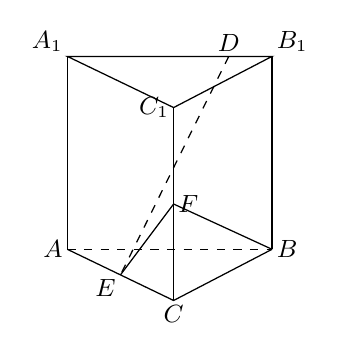
\begin{tikzpicture}[font=\small,line width=0.45pt,
  every node/.style={inner sep=1.5pt}]
  \coordinate (A1) at (0,2.8);  \coordinate (B1) at (2.6,2.8);
  \coordinate (C1) at (1.35,2.15);
  \coordinate (A) at (0,0.35); \coordinate (B) at (2.6,0.35);
  \coordinate (C) at (1.35,-0.30);
  \coordinate (D) at (2.05,2.8);
  \coordinate (E) at (0.675,0.025); \coordinate (F) at (1.35,0.925);
  % 上底、侧棱、下底（遮挡的 AB 为虚线）
  \draw (A1)--(B1)--(C1)--cycle;
  \draw (A1)--(A) (B1)--(B) (C1)--(C);
  \draw[dashed] (A)--(B);
  \draw (A)--(C)--(B);
  % 题设线段
  \draw (B)--(F) (E)--(F);
  \draw[dashed] (D)--(E);
  % 点名
  \node[anchor=south east] at (A1) {$A_1$};
  \node[anchor=south west] at (B1) {$B_1$};
  \node[anchor=east] at (C1) {$C_1$};
  \node[anchor=east] at (A) {$A$};
  \node[anchor=west] at (B) {$B$};
  \node[anchor=north] at (C) {$C$};
  \node[anchor=south] at (D) {$D$};
  \node[anchor=north east] at (E) {$E$};
  \node[anchor=west] at (F) {$F$};
\end{tikzpicture}
\end{center}
\nopagebreak[4]
（1） 证明：$BF\perp DE$。

（2） 当 $B_1D$ 为何值时，面 $BB_1C_1C$ 与面 $DEF$ 所成的二面角正弦值最小？

\Needspace{4\baselineskip}
\textbf{解析}

\Needspace{5\baselineskip}
建立直角坐标系，令 $A=(0,0,0)$，$B=(2,0,0)$，$A_1=(0,0,2)$，$B_1=(2,0,2)$。直三棱柱的侧棱平行于 $z$ 轴。由 $BF\perp A_1B_1$ 且 $A_1B_1\parallel AB$，得 $C$ 的 $x$ 坐标为 $2$；结合 $BC=2$，可取 $C=(2,2,0)$。因此
\nopagebreak[4]
\[
E=(1,1,0),\qquad F=(2,2,1).
\]

\gksubpart{(1)}

\Needspace{5\baselineskip}
设 $D=(d,0,2)$。则
\nopagebreak[4]
\[
\overrightarrow{BF}=(0,2,1),\qquad
\overrightarrow{DE}=(1-d,1,-2),
\]
故 $\overrightarrow{BF}\cdot\overrightarrow{DE}=0+2-2=0$，即 $BF\perp DE$。

\gksubpart{(2)}

\Needspace{5\baselineskip}
设 $t=B_1D$，则 $0\leqslant t\leqslant2$，且 $D=(2-t,0,2)$。平面 $BB_1C_1C$ 为 $x=2$，其法向量可取 $\boldsymbol n_1=(1,0,0)$。由
\nopagebreak[4]
\[
(\overrightarrow{DE})\times(\overrightarrow{DF})
=(3,-1-t,t-2)
\]
\Needspace{5\baselineskip}
可取平面 $DEF$ 的法向量 $\boldsymbol n_2=(3,-1-t,t-2)$。设两平面夹角为 $\theta$，则
\nopagebreak[4]
\[
\sin^2\theta
=1-\frac{(\boldsymbol n_1\cdot\boldsymbol n_2)^2}{|\boldsymbol n_1|^2|\boldsymbol n_2|^2}
=\frac{(t+1)^2+(t-2)^2}{9+(t+1)^2+(t-2)^2}.
\]
令 $N=(t+1)^2+(t-2)^2=2(t-\tfrac12)^2+\tfrac92$。函数 $N/(N+9)$ 随 $N$ 增大而增大，所以最小值在 $t=\tfrac12$ 取得，即 $B_1D=\tfrac12$。

\gkanswer{答案（1）：见解析版}

\gkanswer{答案（2）：$B_1D=\dfrac12$。}

\end{answer}
\begin{answer}
\gksolhead{20}{}

\textbf{题目}（12 分）：

抛物线 $C$ 的顶点为坐标原点 $O$，焦点在 $x$ 轴上，直线 $l:x=1$ 交 $C$ 于 $P$，$Q$ 两点，且 $OP\perp OQ$。已知点 $M(2,0)$，且圆 $M$ 与 $l$ 相切。

（1） 求 $C$，圆 $M$ 的方程。

（2） 设 $A_1$，$A_2$，$A_3$ 是 $C$ 上的三个点，直线 $A_1A_2$，$A_1A_3$ 均与圆 $M$ 相切。判断 $A_2A_3$ 与圆 $M$ 的位置关系，并说明理由。

\Needspace{4\baselineskip}
\textbf{解析}

\gksubpart{(1)}

\Needspace{5\baselineskip}
焦点在 $x$ 轴上的抛物线可设为 $y^2=4px$。直线 $x=1$ 上的交点为 $P=(1,2\sqrt p)$、$Q=(1,-2\sqrt p)$。由 $OP\perp OQ$，
\nopagebreak[4]
\[
(1,2\sqrt p)\cdot(1,-2\sqrt p)=1-4p=0,
\]
得 $p=1/4$，所以 $C:y^2=x$。

圆心 $M=(2,0)$，圆与直线 $x=1$ 相切，半径为 $1$，故圆方程为 $(x-2)^2+y^2=1$。

\gksubpart{(2)}

\Needspace{5\baselineskip}
用参数表示抛物线点为 $P(u)=(u^2,u)$。过 $P(u),P(v)$ 的弦方程为
\nopagebreak[4]
\[
x-(u+v)y+uv=0.
\]
\Needspace{5\baselineskip}
它与圆心 $M=(2,0)$、半径 $1$ 的圆相切，当且仅当圆心到直线的距离为 $1$，即
\nopagebreak[4]
\[
(2+uv)^2=1+(u+v)^2.
\]
\Needspace{5\baselineskip}
固定 $u$，该条件是关于 $v$ 的二次方程
\nopagebreak[4]
\[
(u^2-1)v^2+2uv+(3-u^2)=0.
\]
\Needspace{5\baselineskip}
其两根为 $v,w$，由韦达定理
\nopagebreak[4]
\[
v+w=-\frac{2u}{u^2-1},\qquad vw=\frac{3-u^2}{u^2-1}.
\]
\Needspace{5\baselineskip}
因此弦 $A_2A_3$ 的方程为 $x-(v+w)y+vw=0$。代入圆心距公式：
\nopagebreak[4]
\[
\frac{|2+vw|}{\sqrt{1+(v+w)^2}}
=\frac{(u^2+1)/|u^2-1|}{(u^2+1)/|u^2-1|}=1.
\]
所以 $A_2A_3$ 也与圆 $M$ 相切。

\gkanswer{答案（1）：$C:y^2=x$，圆 $M:(x-2)^2+y^2=1$。}

\gkanswer{答案（2）：$A_2A_3$ 与圆 $M$ 相切。}

\end{answer}
\begin{answer}
\gksolhead{21}{}

\textbf{题目}（12 分）：

已知 $a>0$ 且 $a\ne1$，函数 $f(x)=\dfrac{x^a}{a^x}\ (x>0)$。

（1） 若 $a=2$，求 $f(x)$ 的单调区间。

（2） 若曲线 $y=f(x)$ 与直线 $y=1$ 有且仅有两个交点，求 $a$ 的取值范围。

\Needspace{4\baselineskip}
\textbf{解析}

\Needspace{5\baselineskip}
对 $f(x)=x^a/a^x$ 取对数：
\nopagebreak[4]
\[
\ln f(x)=a\ln x-x\ln a,\qquad
\frac{f'(x)}{f(x)}=\frac ax-\ln a.
\]

\gksubpart{(1)}

当 $a=2$ 时，导数符号由 $2/x-\ln2$ 决定。它在 $0<x<2/\ln2$ 时为正，在 $x>2/\ln2$ 时为负，因此递增区间为 $(0,2/\ln2)$，递减区间为 $(2/\ln2,+\infty)$。

\gksubpart{(2)}

若 $0<a<1$，则 $\ln a<0$，所以 $a/x-\ln a>0$，函数从 $0$ 严格递增至 $+\infty$，与 $y=1$ 只有一个交点。

\Needspace{5\baselineskip}
若 $a>1$，函数在 $x=a/\ln a$ 处取得唯一最大值
\nopagebreak[4]
\[
f_{\max}=\left(\frac{a}{e\ln a}\right)^a,
\]
且在 $x\to0^+$ 和 $x\to+\infty$ 时均趋于 $0$。因此恰有两个交点当且仅当 $a/(e\ln a)>1$。令 $s=\ln a>0$，条件等价于 $e^{s-1}>s$；由指数函数的凸性（或考察 $e^{s-1}-s$ 的导数），该式对 $s>0$ 成立，等号仅在 $s=1$。故需 $a>1$ 且 $a\ne e$。

\gkanswer{答案（1）：增区间为 $\left(0,\dfrac2{\ln2}\right)$，减区间为 $\left(\dfrac2{\ln2},+\infty\right)$。}

\gkanswer{答案（2）：$a\in(1,e)\cup(e,+\infty)$。}

\end{answer}
\begin{answer}
\gksolhead{22}{}

\textbf{题目}（10 分）选修 4—4：坐标系与参数方程：

在直角坐标系 $xOy$ 中，以坐标原点为极点，$x$ 轴正半轴为极轴建立极坐标系，曲线 $C$ 的极坐标方程为 $\rho=2\sqrt2\cos\theta$。

（1） 将 $C$ 的极坐标方程化为直角坐标方程。

（2） 设点 $A$ 的直角坐标为 $(1,0)$，$M$ 为 $C$ 上的动点，点 $P$ 满足 $\overrightarrow{AP}=\sqrt2\,\overrightarrow{AM}$。写出 $P$ 的轨迹 $C_1$ 的参数方程，并判断 $C$ 与 $C_1$ 是否有公共点。

\Needspace{4\baselineskip}
\textbf{解析}

\gksubpart{(1)}

\Needspace{5\baselineskip}
由 $x=\rho\cos\theta$、$\rho^2=x^2+y^2$，
\nopagebreak[4]
\[
\rho=2\sqrt2\cos\theta
\quad\Longrightarrow\quad
x^2+y^2=2\sqrt2\,x,
\]
即 $(x-\sqrt2)^2+y^2=2$。

\gksubpart{(2)}

\Needspace{5\baselineskip}
令 $M=(\sqrt2+\sqrt2\cos t,\sqrt2\sin t)$，这是圆 $C$ 的参数方程。由 $\overrightarrow{AP}=\sqrt2\,\overrightarrow{AM}$ 且 $A=(1,0)$，
\nopagebreak[4]
\[
P=A+\sqrt2(M-A),
\]
\Needspace{5\baselineskip}
所以
\nopagebreak[4]
\[
x=3-\sqrt2+2\cos t,\qquad y=2\sin t,\qquad 0\leqslant t<2\pi.
\]
轨迹 $C_1$ 的圆心为 $(3-\sqrt2,0)$、半径为 $2$；$C$ 的圆心为 $(\sqrt2,0)$、半径为 $\sqrt2$。两圆心距为 $|3-2\sqrt2|<2-\sqrt2$，小于半径差，故 $C$ 完全位于 $C_1$ 内且不相切，两曲线没有公共点。

\gkanswer{答案（1）：$(x-\sqrt2)^2+y^2=2$。}

\gkanswer{答案（2）：$C_1$ 的参数方程为 $\begin{cases}x=3-\sqrt2+2\cos t,\\y=2\sin t,\end{cases}\ t\in[0,2\pi)$；$C$ 与 $C_1$ 无公共点。}

\end{answer}
\begin{answer}
\gksolhead{23}{}

\textbf{题目}（10 分）选修 4—5：不等式选讲：

已知函数 $f(x)=|x-2|$，$g(x)=|2x+3|-|2x-1|$。
\nopagebreak[4]
\begin{center}% 2021 全国甲卷理科 23：不等式作图用的空白方格坐标系
% 源图为以原点为中心、横纵各 8 格的网格，只标坐标轴、O 与单位刻度。
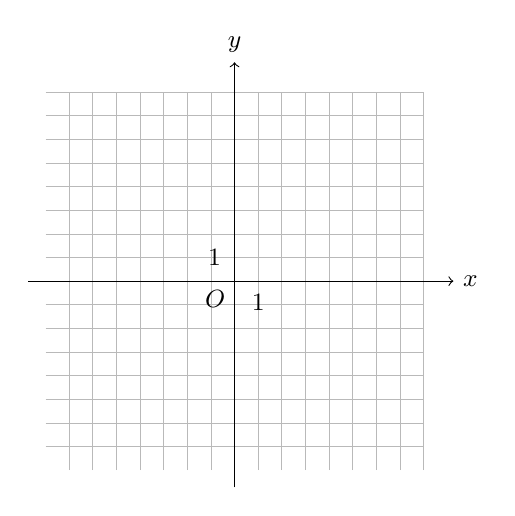
\begin{tikzpicture}[font=\small,line width=0.4pt]
  \def\u{0.30}
  \draw[gray!55,line width=0.25pt] (-2.4,-2.4) grid[step=\u] (2.4,2.4);
  \draw[->] (-2.62,0)--(2.78,0) node[anchor=west] {$x$};
  \draw[->] (0,-2.62)--(0,2.78) node[anchor=south] {$y$};
  \node[anchor=north east,inner sep=2pt] at (-0.04,-0.04) {$O$};
  \node[anchor=north,inner sep=3pt] at (\u,-0.06) {$1$};
  \node[anchor=east,inner sep=3pt] at (-0.06,\u) {$1$};
\end{tikzpicture}
\end{center}
\nopagebreak[4]
（1） 画出 $y=f(x)$ 和 $y=g(x)$ 的图象。

（2） 若 $f(x+a)\geqslant g(x)$，求 $a$ 的取值范围。

\clearpage

\Needspace{4\baselineskip}
\textbf{解析}

\gksubpart{(1)}

$y=f(x)$ 为顶点 $(2,0)$ 的 V 形；$g(x)$ 在 $x\leqslant-\dfrac32$ 时为 $-4$，在 $[-\dfrac32,\dfrac12]$ 上为 $4x+2$，在 $x\geqslant\dfrac12$ 时为 $4$，据此在题图网格作图。

\gksubpart{(2)}

说明：原题未明示量词，以下分别讨论全称与存在两种解释。

全称解释下，当 $x\geqslant\dfrac12$ 时 $g(x)=4$，且 $\min_{x\geqslant1/2}|x+a-2|=\max(0,a-\dfrac32)$，故必要地 $a\geqslant\dfrac{11}{2}$。反之若 $a\geqslant\dfrac{11}{2}$，则 $x\leqslant-\dfrac32$ 时 $g=-4\leqslant f$；在 $[-\dfrac32,\dfrac12]$ 与 $[\dfrac12,+\infty)$ 上，$f(x+a)-g(x)$ 分别为 $a-4-3x$ 与 $x+a-6$，均不小于 $a-\dfrac{11}{2}\geqslant0$。故全称解释的范围为 $a\in[\dfrac{11}{2},+\infty)$。存在解释下取任意 $x\leqslant-\dfrac32$，即有 $g(x)=-4\leqslant0\leqslant f(x+a)$，故范围为 $\mathbf R$。

\gkanswer{答案（1）：$y=|x-2|$；$g(x)=-4$（$x\leqslant-\dfrac32$）、$4x+2$（$-\dfrac32\leqslant x\leqslant\dfrac12$）、$4$（$x\geqslant\dfrac12$）。}

\gkanswer{答案（2）：全称解释为 $a\in\left[\dfrac{11}{2},+\infty\right)$；存在解释为 $a\in\mathbf R$。}

\end{answer}